%!TEX root = ../../../../thesis.tex
\section{Natural Computing}

	For some time the word \emph{Nature} and \emph{Computing} used to denote terms which could hardly be any more opposite to each other. Starting with the mid 1940s this perception began to fade gradually when researchers started to explore the exciting possibility of looking towards nature for alternative ways of doing computing. The search for new problem solving techniques, novel approaches to synthesize natural phenomena in silico as well as novel natural materials to perform computation began. Today, the pursuit of these three distinct, yet interrelated approaches is known as \emph{Natural Computing}~\cite{de2005natural,de2006fundamentals}.

	In this section we give a short introduction to the scope of Natural Computing and mention its most important areas of interest. Our exposition closely follows de~Castro~\cite{de2007fundamentals} who describes natural computing as the extraction of ideas from nature to develop computational systems, or using natural materials to perform computation. He suggest to divide the field into three main areas:

	\begin{description}
		\item[a)] Computing inspired by nature
		\item[b)] The simulation and emulation of nature by means of computing
		\item[c)] Computing with natural materials
	\end{description}

	\begin{figure}
			\centering
			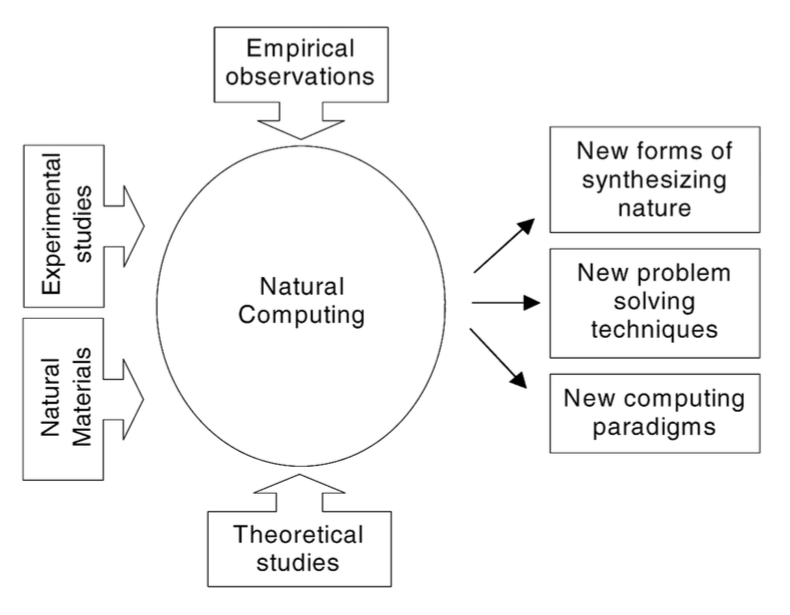
\includegraphics[width=\oneimagewide,keepaspectratio]{natural_computing.png}
			\caption[The goals of natural computing.]{A schematic of the components and goals of natural computing.}
			\label{fig:natural_computing}
	\end{figure}

	\Fref{fig:natural_computing} illustrates the goals of natural computing. The study of these three highly entangled areas seamlessly merge empirical observations and theoretical studies from diverse fields such as biology, physics, chemistry, engineering and computer science amongst others. Thus it is vital for researchers to be open, collaborate and share their ideas and knowledge in order to meet the challenges posed by the highly interdisciplinary field that is natural computing.

	What follows is a short description of the main areas of natural computing including some of its most important achievements. For an extensive discussion and a comprehensive collection of references see~\cite{de2007fundamentals}.

	\FloatBarrier

	\subsection{Computing Inspired by Nature}

		In the area of natural computing, the goal is to utilize natural processes and phenomena as a source of inspiration in order to devise novel computational systems and algorithms geared towards solving complex problems. Of particular interest are alternative solution methods to classes of problems for which resolution remains difficult for standard techniques such as linear, non-linear and dynamic programming. Some of the best known representatives of nature inspired computing include artificial neural networks\footnote{Artificial neural networks focus on solving computational problems as opposed to the accurate biological modeling of the brain and the nervous system. The latter are questions of computational neuroscience.}, evolutionary algorithms and swarm intelligence~\cite{de2007fundamentals}.

		\begin{description}
			
			\item[Neural networks] are formed by \emph{artificial neurons} arranged according to a predefined network architecture, typically consisting of several functional layers of neurons. Triggered by a special \emph{activation function}, each neuron may fire, \ie mapping its potentially many weighted inputs to a single output. Different types of \emph{learning strategies} may adjust the input weights of each neuron in response to encountered input stimuli. Indeed, some amount of learning, also known as training, is typically required before a neural network becomes competent. They can however, be efficiently trained to do various tasks such as classification, pattern recognition or more general function approximation. Unfortunately, a deeper understanding of why neuronal networks work the way they do remains elusive. A fact, that does not diminish their usefulness which lead to their large (commercial) success. For references see~\cite{Haykin:1998:NNC:521706,Fausett:1994:FNN:197023,Bishop:1995:NNP:525960}.

			\item[Evolutionary Computing] and in particular genetic algorithms, try to leverage the power of natural evolution by simulating a population of individuals with certain traits. Individuals represent points in a search space associated with solutions to a given optimization problem. Each potential solution is evaluated with regards to the objective function of the problem. This process is also known as determining the \emph{fitness} of an individual. Individuals are then selected to reproduce, \ie pass on their traits to the next generation, with a probability proportional to their fitness in an sexual or asexual fashion. In the former case the offspring is determined by a recombination of the traits of the parents. Further genetic variations is introduced by random mutation of traits. If this process is repeated it evolves towards better solutions in an iterative manner. Typically such algorithms terminate after a predefined number of iterations or when the desired level of fitness was reached. Evolutionary algorithms have found success in problems such as routing, scheduling, packing and various machine learning tasks~\cite{Back:1997:HEC:548530,spears1993overview,zitzler2000comparison}. Important practical applications include determining optimal design choices in various engineering settings~\cite{Schwefel:1993:EOS:529401,kicinger2005evolutionary}.

			\item[Swarm Intelligence] encompasses techniques for problem solving that are inspired by the collective behavior of human or animal societies. They rely on the social behavior of a population of individuals capable of interacting with the environment or one another in either a direct or indirect fashion~\cite{de2007fundamentals}. The popular \emph{ant colony optimization} approach uses artificial ants that lay or follow artificial \emph{pheromone trails}. In the shortest path problem for instance, ants travel all possible paths between two distinct nodes at the beginning. However, as time goes by, longer routes will have less pheromones associated with them due to pheromones evaporating. Since the probability for an ant to choose a given route is proportional to the present amount of pheromone, ants become less likely to travel long routes and tend to concentrate on the shorter paths which thus gets reinforced repeatedly. As a result, ants are progressively converging towards the shortest path. This general scheme can be adapted to various other discrete optimization problems such as the traveling salesman problem and certain vehicle and network routing problems. For references see~\cite{bonabeau2000swarm,bonabeau2000inspiration,Bonabeau:1999:SIN:328320,fukuyama2008fundamentals}.
			
		\end{description}

		\FloatBarrier

	\subsection{Synthesis of Nature by Means of Computing}
		
		The synthesis of nature by means of computing aims for full or partial reproduction of phenomena, behaviors or patterns observed in nature~\cite{de2007fundamentals}. This \emph{in silico} approach allows the exploration of a wide range of questions which may not be tractable using traditional analytic or experimental techniques. Frequently theoretical work proposes theories and models to be studied using simulations with the aim of obtaining a deeper understanding of the original phenomenon being modeled. The simulation itself may serve as an evaluation of a proposed model, ideally suggesting further improvements to the models and itself. In addition to the enormous increase in computing power observed in the last few decades, much of the success of fields like computational biology, computational chemistry or computational physics owes to the symbiotic relationship between theory and simulation.

		Examples for the synthesis of natural phenomena include \emph{cellular automata} as a model for self-reproduction or \emph{L-systems} modeling the development of multicellular organisms. These concepts were designed to capture and study certain, well-defined rules and associated behavior. However, over time their elegance and simplicity lead to a variety of unforeseen applications. Cellular automata have played a role in modeling the physics of fluids or gases on lattices~\cite{rothman2004lattice} and the microscopic study of high-way traffic~\cite{nagel1998two} to name but a few. L-systems have been a successful tool in the study of various properties of \emph{virtual plants}~\cite{tardieu2003virtual}. In addition to that they have found applications outside of biology in formal language theory, the study of tumor growth and even musical composition~\cite{de2005natural}.

		Arguably the most exciting field we like to mention in the context of synthesis by means of computing is the study of \emph{artificial life}~\cite{Langton:1995:ALO:526815}. Within artificial life, it is proposed that life itself should be regarded as an emergent property resulting from the organization of matter as opposed to a simple property of the matter itself. It follows that besides the carbon based chain of life observed on earth, \ie \emph{life-as-we-know-it}, different materials could lead to alternative life-like organizations aptly termed \emph{life-as-could-be}. While it is debatable what properties such an organization needs to have to be rightfully termed alive, the prospect of new unknown forms of life is exciting. 

		A well-known example for non-trivial behavior in the context of life-as-could-be is demonstrated by \emph{boids}~\cite{Reynolds:1987:FHS:37401.37406}. Here artificial life is represented merely as virtual agents that are allowed to move in space. They obey the following simple rules: (1) Avoid collision with neighboring boids or obstacles; (2) Match velocity and direction of neighboring boids; (3) Stay close to neighboring boids. From these simple rules complex collective behavior emerges allowing a flock of boids to closely imitate the non-trivial behavior seen in flocking birds or shoals of fish~\cite{de2007fundamentals}.

		The examples in this section illustrate that much can be learned from attempts to synthesize nature by means of computing. It is likely that ongoing research efforts will sooner or later drastically alter our understanding of nature in general and life in particular. It is my personal opinion that the question of how life arises from inanimate matter constitutes one of the most important scientific questions in the entire history of science.

		For extensive reviews on the topic of artificial life, we refer the reader to~\cite{Langton:1995:ALO:526815,Boden:1996:PAL:525139,bedau2000open,taylor1993artificial}.

		\FloatBarrier

	\subsection{Computing with natural materials}

		Computing with natural materials aims to go beyond standard transistor-based computing by utilizing natural materials other than silicon as media for computing. Examples for approaches to computing that are in stark contrast to conventional computing are DNA and quantum computing~\cite{de2007fundamentals}. 

		In \emph{DNA computing} complex molecules such as DNA strands are used to store and process information. Complex computations can then be realized using a set of basic operations that apply to interacting molecules. These operations are derived from molecular biology and involve fusing, copying or deletion of DNA strands to name but a few. The power of DNA computing derives from the fact that a large number of molecules may interact with each other simultaneously. Despite the potentially slow individual reactions, the inherent massive parallel information processing capability of DNA computing lead to novel approaches to hard combinatorial problems such as the Hamiltonian path problem~\cite{adleman1994molecular}. Today various other applications are known ranging from matrix multiplication to cryptography~\cite{puaun2000computing,boneh1996computational,lipton1996breaking,oliver1998computation}. Drawbacks of DNA computing include scaling with problem size as well as retrieving the actual solution for a problem proposed by a DNA computation~\cite{de2007fundamentals}.

		Another promising alternative to classical computing is \emph{quantum computing}~\cite{Nielsen:2011:QCQ:1972505}. Here the so-called \emph{qubit} replaces the classic binary bit which is limited to two states, zero or one. In contrast to that, the qubit, thanks to its quantum nature, can represent any superposition state representing all possible combinations of zero and one simultaneously. Thus, a quantum computer using $n$ qubits may be in $2^n$ different states at the same time unlike a classical computer which is in exactly one state at a time. Elementary operation on qubits take the form of quantum logic gates. Gates may be arranged in such a way that they compute the solution to a given problem. A sequence of gates operating on qubits is then called a quantum algorithm. In the final steps of any quantum algorithm the qubit superposition is collapsed in order to obtain the result which is often probabilistic. Exploiting the massive in-build parallelism, dedicated quantum algorithms have been developed that outperform all known classical algorithms for a given problem. The two most prominent ones being Shor's integer factorization and Grovers's database search algorithm~\cite{shor1999polynomial,grover1996fast}. In addition to speeding up certain tasks, quantum systems may operate in ways that classical systems cannot. This fact is exploited in \emph{quantum communication} or \emph{quantum cryptography}, where protocols have been developed that reduce communication complexity or provide perfect secrecy~\cite{de2007fundamentals}. A major roadblock on the way of success for quantum computing consists of the physical realization of coherent systems capable of preparing qubits and executing quantum algorithms reliably. Here the very quantum properties that enable extraordinary computation, present formidable difficulties when it comes to controlling the quantum system. Unfortunately this fact still severely limits the number of qubits that have been used in successful computing applications~\cite{Nielsen:2011:QCQ:1972505}. 

		\FloatBarrier
